\documentclass[serif,xcolor=pdftex,dvipsnames,table,hyperref={bookmarks=false,breaklinks}]{beamer}

%%%%%%%%%%%%%%%%
% Change the macros below to configure the title slides
% for your course.
\newcommand{\coursename}{COMPSCI 590N}
\newcommand{\instructor}{Roy J. Adams}
\newcommand{\university}{University of Massachusetts Amherst}
\newcommand{\department}{College of Information and Computer Sciences}
%%%%%%%%%%%%%%%%

\newcommand\HUGE{\@setfontsize\Huge{50}{60}}

\newcommand{\settitlecard}[2]{
  \title[\coursename  Lecture #1] 
    {\coursename \\ Lecture #1: #2}
     \author[\instructor]{\instructor}
     \institute[\university]{
     \department\\
     \university
   }
\date{}
}

\newcommand{\maketitlepage}{
  \begin{frame}
  \titlepage
  %\center{
    %If you use the slides unmodified, retain the attribution below
  %  \tiny{Slides by Roy J. Adams (rjadams@cs.umass.edu). 
    %If you modify the slides, please retain the alternate attribution below
    %\tiny{Based on slides by Roy J. Adams (rjadams@cs.umass.edu). \\    
  %  }                                              
  %}  
  \end{frame}
}

\AtBeginSection[]
{
  \begin{frame}<beamer>{Outline}
    \tableofcontents[currentsection,subsectionstyle=hide]
  \end{frame}
}


\newcommand{\cut}[1]{}

\newcommand{\iconbox}[4]{
  \only<#1-#2>{
    \begin{columns}[T]
      \column{0.5in}
           \includegraphics[width=0.5in]{#3}
       \column{3.7in}
            #4
    \end{columns}
    \medskip
    \medskip
    \medskip
  }
}

\mode<presentation>{
  \usepackage{../beamertheme589theme}
  \setbeamercovered{invisible}
}

\mode<handout>{
  \usepackage{../beamertheme589theme}
  \setbeamercovered{transparent}
}


\usepackage[english]{babel}
\usepackage[latin1]{inputenc}
\usepackage{times}
\usepackage[T1]{fontenc}
\usepackage{amsmath}
\usepackage{amssymb}
\usepackage[noend]{algorithmic}
\usepackage{algorithm}
\usepackage{listings}
\usepackage{tcolorbox}
\usepackage{xmpmulti}

\renewcommand\mathfamilydefault{\rmdefault}

\newcommand{\setA}{\mathcal{A}}
\newcommand{\setB}{\mathcal{B}}
\newcommand{\setS}{\mathcal{S}}
\newcommand{\setV}{\mathcal{V}}
\DeclareMathOperator*{\union}{\bigcup}
\DeclareMathOperator*{\intersection}{\bigcap}
\DeclareMathOperator*{\Val}{Val}
\newcommand{\mbf}[1]{{\mathbf{#1}}}
\DeclareMathOperator*{\argmax}{arg\,max}
\DeclareMathOperator*{\argmin}{arg\,min}
\DeclareMathOperator*{\sign}{sign}
\newcommand{\deriv}[2]{\frac{\partial{#1}}{\partial{#2}}}

\lstdefinestyle{custompython}{
  belowcaptionskip=1\baselineskip,
  breaklines=true,
  frame=single,
  xleftmargin=\parindent,
  language=Python,
  showstringspaces=false,
  basicstyle=\footnotesize\ttfamily,
  keywordstyle=\bfseries\color{green!40!black},
  commentstyle=\itshape\color{purple!40!black},
  identifierstyle=\color{blue},
  stringstyle=\color{orange},
}
\lstset{style=custompython}

\makeatletter
\renewcommand*\env@matrix[1][*\c@MaxMatrixCols c]{%
  \hskip -\arraycolsep
  \let\@ifnextchar\new@ifnextchar
  \array{#1}}
\makeatother

\newcommand\norm[1]{\left\lVert#1\right\rVert}


\settitlecard{10}{Probability 2}

\begin{document}

\maketitlepage

% \section{Announcements}
% \subsection{Foo}
%
% \begin{frame}[t]{Announcements}
% \end{frame}

\section{Visualizing Distributions}
\subsection{Foo}

\begin{frame}[t]{Histograms and Counting}
	\begin{itemize}[<+->]
		\item An important tool for exploring data is visualizing the distribution it came from.
		\begin{itemize}[<+->]
			\item Allows us to verify and inform modeling decisions.
			\item Summary statistics (e.g. mean, standard deviation, skewness, kurtosis, etc.), while important and useful, discard information about the data.
		\end{itemize}
		\item A flexible tool for visualizing data distributions is the histogram.
	\end{itemize}
	\pause
	\centering
	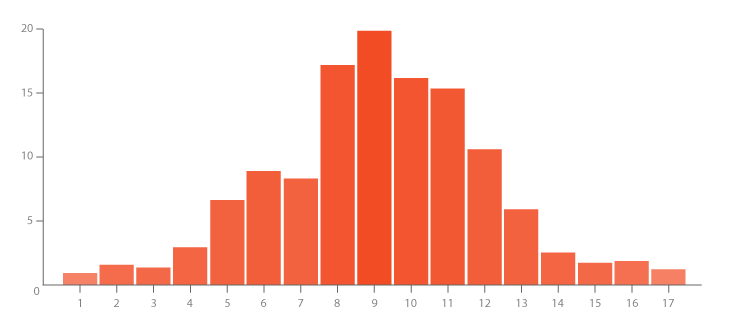
\includegraphics[height=1in]{{../Figures/histogram}.png}
\end{frame}

\begin{frame}[t,fragile]{Histograms and Counting}
	% Numpy functions
	Numpy provides functions for counting and computing histograms.
	
	\begin{lstlisting}
		>>> import numpy as np
		>>> A = np.random.randn(1000)
		>>> np.histogram(A,nbins=5)
		>>> counts,bin_edges = np.histogram(A,bins=7)
		>>> counts
		array([ 38, 180, 381, 289,  98,  11,   3])
		>>> bin_edges
		array([-2.75925765, -1.77917762, -0.7990976 ,  0.18098242,  1.16106244,
		        2.14114246,  3.12122248,  4.1013025 ])
	\end{lstlisting}
\end{frame}

\begin{frame}[t,fragile]{Histograms in Python}
	\begin{itemize}[<+->]
		\item There are a variety of tools for plotting distributions:
		\begin{itemize}[<+->]
			\item \verb|matplotlib.pyplot.histogram| computes and plots a histogram from an array.
			\item \verb|pandas.DataFrame.hist| plots a histogram directly from a \verb|pandas.DataFrame|.
			\item \verb|Seaborn| is an extension to \verb|matplotlib| design explicitly for plotting distributions.
		\end{itemize}
	\end{itemize}
	% Seaborn Demo
\end{frame}

\section{Sampling}
\subsection{Foo}

\begin{frame}[t]{Applications of Randomness}
	Randomness is a core operation for many commonly used algorithms:
	\pause
	\begin{itemize}[<+->]
		\item Cryptography and encryption.
		\item Randomized storage (e.g. random hash tables used in Python dictionaries).
		\item Randomized communications (e.g. LAN).
		\item Approximate integration (we will look at this later).
		\item Randomized experiments.
		\item Statistical modeling:
		\begin{itemize}[<+->]
			\item Evaluating models.
			\item Approximate inference.
			\item Approximate estimation.
		\end{itemize}
		\item \textbf{Many} other randomized algorithms.
	\end{itemize}
\end{frame}

\begin{frame}[t]{Random Sampling}
	\begin{itemize}[<+->]
		\item Problem: Given a distribution $p(x)$ we would like to generate samples from this distribution.
		\item Example: To generate samples from a Bernoulli distribution (binary), flip a bunch of coins. The result of each coin flip is a sample from the Bernoulli.
	\end{itemize}
\end{frame}

\begin{frame}[t]{Types of Sampling}
	As you might imagine, sampling has been the focus of intense study for a long time. Some common sampling algorithms are:
	\pause
	\begin{itemize}[<+->]
		\item Inverse CDF sampling (we will look at this algorithm).
		\item Rejection sampling.
		\item Markov Chain Monte Carlo (MCMC).
		\item Metropolis-Hastings.
		\item Slice sampling.
		\item The list goes on.
	\end{itemize}
\end{frame}

\begin{frame}[t]{Cumulative Distribution Functions}
	Given a distribution $p(x)$ for a random variable $X$, the associated Cumulative Distribution Function (CDF) $F(x)$, gives the probability that $X$ is less then some value, i.e. $F(x) = P(X \leq x)$.
	
	\pause
	\begin{block}{Cumulative Distribution Function}
		The CDF $F(x)$ for a distribution $p(x)$ is given by,
		
		$$F(x) = \int_{-\infty}^x p(x') dx'$$
		
		for continuous variables and by
		
		$$F(x) = \sum_{x' = -\infty}^{x} P(x')$$
		
		for discrete variables.
	\end{block}
\end{frame}

\begin{frame}[t]{Cumulative Distribution Functions: Multinomial}
	For example: Consider the CDF for $Multinomial(1,\frac{1}{6},...,\frac{1}{6})$ (i.e. a six sided dice roll).
	\pause
	\begin{align*}
		F(x) &= P(X \leq x) = \sum_{i = 1}^{x} \frac{1}{6}\\
		F(3) &= P(X \leq 3) = \frac{3}{6} = \frac{1}{2}
	\end{align*}
	
	\pause
	% multinomial CDF
\end{frame}

\begin{frame}[t]{Sampling Algorithms: Inverse CDF Sampling}
	One of the most fundamental sampling algorithms is inverse CDF sampling. For any invertible CDF, we can use the following algorithm.
	\pause
	\begin{block}{Inverse CDF Sampling}
		Let $F(x)$ be an invertible CDF. Then we can sample from the associated distribution by:
		\begin{enumerate}
			\item Sample $u^{(s)}$ from a Uniform(0,1).
			\item $x^{(s)} = F^{-1}(U)$
		\end{enumerate}
	\end{block}
\end{frame}

% \begin{frame}[t]{Sampling Algorithms: Inverse CDF Sampling}
% 	% Multinomial
% \end{frame}
%
% \begin{frame}[t]{Sampling Algorithms: Inverse CDF Sampling}
% 	% Gaussian
% \end{frame}


\begin{frame}[t]{Monte Carlo Integration}
	\begin{itemize}[<+->]
		\item \textbf{Monte Carlo Integration} is a method for approximating the value of an integral that is difficult (or impossible) to compute.
		\item The core idea is based on approximating \textbf{expected values}.
	\end{itemize}
\end{frame}

\begin{frame}[t]{Expected Values}
	A common computation when working with probability distributions is an expected value.
	
	\pause
	\begin{block}{Expected Value}
		Given a distribution $p(x)$ over a random variable $X$ and a function of the random variable $f:\Omega\to \mathbb{R}$, the expected valued of the function is defined as
		
		$$\mathbb{E}[f(X)] = \int_\Omega p(x)f(x)dx$$
		
		where the integral is a sum when $X$ is discrete.
	\end{block}
\end{frame}

\begin{frame}[t]{Expected Values: Multinomial}
	\begin{itemize}[<+->]
		\item Let $X$ be the result of a fair six-sided dice roll.
		\item What is $\mathbb{E}[X]$?
	\end{itemize}
	
	\pause
	\begin{align*}
		\mathbb{E}[X] &= \sum_x P(X=x)\cdot X\\
		&= \sum_{x=1}^6 \frac{1}{6}\cdot x\\
		&= \frac{1}{6}(1+2+3+4+5+6) = 3.5
	\end{align*}
\end{frame}

\begin{frame}[t]{Expected Values: Normal}
	\begin{itemize}[<+->]
		\item Let $X$ be a Normally distributed random variable with mean $\mu$ and standard deviation $\sigma$.
		\item What is $\mathbb{E}[X^2]$?
	\end{itemize}
	\pause
	\begin{align*}
		\mathbb{E}[X^2] &= \int_x \frac{1}{\sigma\sqrt{2\pi}}\exp\left(-\frac{(x-\mu)^2}{2\sigma^2}\right)x^2 dx\\
		&= \frac{1}{\sigma\sqrt{2\pi}}\int_x \exp\left(-\frac{(x-\mu)^2}{2\sigma^2}\right)x^2 dx\\
		&= \frac{1}{\sigma\sqrt{2\pi}}\int_x \exp\left(-\frac{(x-\mu)^2}{2\sigma^2}\right)x^2 dx\\
	\end{align*}
\end{frame}

\begin{frame}[t]{The Importance of Expected Values}
\end{frame}

\begin{frame}[t]{Difficult Expected Values}
	\begin{itemize}[<+->]
		\item In many cases, the expected value is too complex to evaluate.
		\item This may occur because:
		\begin{itemize}[<+->]
			\item The normalization constant of the distribution is difficult to evaluate.
			\item There is not analytical solution to the integral.
		\end{itemize}
		\item What do we do? Approximate!
		\item Types of approximations:
		\begin{enumerate}[<+->]
			\item Approximate the distribution with a simpler one that allows us to take the expectation (e.g. Variational Bayes).
			\item Upper and lower-bound based approximations (e.g. Variational Approximations).
			\item Sampling based approximations (Monte Carlo Integration).
		\end{enumerate}
	\end{itemize}
\end{frame}

\begin{frame}[t]{Monte Carlo Integration}
	\textbf{Monte Carlo integration} approximates an expected value by sampling from the associated distribution and then taking an average.
	\pause
	\begin{block}{Monte Carlo Integration}
		Let $X$ be a random variable drawn from $p(x)$, let $f(x)$ be a function of $X$, and let $x^{(1)},...,x^{(S)}$ be samples from $p(x)$, then
		
		$$\mathbb{E}(f(x)) \approx \frac{1}{S}\sum_s x^{(s)}$$
	\end{block}
\end{frame}

% \begin{frame}[t]{Monte Carlo Integration: Mean of a Normal}
%
% \end{frame}
%
% \begin{frame}[t]{Monte Carlo Integration: Variance of a Normal}
%
% \end{frame}

\begin{frame}[t]{Monte Carlo Integration}
	How can we use Monte Carlo integration to calculate general integrals?
	
	\pause
	\begin{align*}
		\int_a^b f(x) dx &= \int_a^b \frac{b-a}{b-a} f(x) dx\\
		&= (b-a) \int_a^b \frac{1}{b-a} f(x) dx\\
		&= (b-a) \mathbb{E}[f(X)]\\
	\end{align*}
	
	where $X$ is draw from $Uniform(a,b)$.
	
	\pause
	\begin{itemize}[<+->]
		\item Now we can approximate this expected value using sampling.
		\item This works for multidimensional integrals as well.
	\end{itemize}
\end{frame}

\begin{frame}[t]{Monte Carlo Integration: Area of a Circle}
	\begin{itemize}[<+->]
		\item How can we use Monte Carlo integration to estimate the area of a circle with radius $r$?
		\item Step 1: Formulate the problem as a bounded integral.
	\end{itemize}
	
	\pause
	A circle is defined by $x^2 + y^2 = r^2$ so we can define a piecewise function that tells us whether we are inside or outside of the circle.
	\begin{align*}
		f(x,y) &= \left\{
			\begin{array}{ll}
				1 & : x^2 + y^2 \leq r^2\\
				0 & : x^2 + y^2 > r^2
			\end{array}
		\right.
	\end{align*}
	\pause
	The area of a circle is given by
	\begin{align*}
		A_r = \int_{-r}^r \int_{-r}^r f(x,y) dx dy
	\end{align*}

\end{frame}

\begin{frame}[t]{Monte Carlo Integration: Area of a Circle}
	\begin{itemize}[<+->]
		\item Now that the area is formulated as an integral, how do we approximate it with sampling?
		\item Step 1: Identify the sampling distribution.
	\end{itemize}
	
	\pause
	\begin{itemize}[<+->]
		\item In this case we are integrating over the $2r \times 2r$ square.
		\item How do we sample uniformly from a square?
		\item Sample $x$ and $y$ independently from $Uniform(-r,r)$
	\end{itemize}
	% plot
	
\end{frame}

\begin{frame}[t]{Monte Carlo Integration: Area of a Circle}
	Now we can estimate the area of a circle as:
	
	\begin{align*}
		A_r &= \int_{-r}^r \int_{-r}^r f(x,y) dx dy\\
		&\approx 2r^2 \frac{1}{S}\sum_s f(x^{(s)},y^{(s)})
	\end{align*}
	
	where
	
	\begin{align*}
		f(x,y) &= = \left\{
			\begin{array}{ll}
				1 & : x^2 + y^2 <= r^2\\
				0 & : x^2 + y^2 > r^2
			\end{array}
		\right.
	\end{align*}
	
\end{frame}

\begin{frame}[t]{Monte Carlo Integration: Area of a Circle}
	% Animation
\end{frame}


\section{Sources of Randomness}
\subsection{Foo}

\begin{frame}[t]{Sources of Randomness}
	\begin{itemize}[<+->]
		\item Most sampling methods are based on the assumption that we can generate a uniform random number.
		\item How do we generate a uniform random number?
		\item There are two main methods:
		\begin{enumerate}[<+->]
			\item Harvested natural randomness
			\item Pseudo-random number generation
		\end{enumerate}
	\end{itemize}
\end{frame}

\begin{frame}[t]{Harvesting Natural Randomness}
	\begin{itemize}[<+->]
		\item The idea behind harvesting natural randomness is that there natural phenomenon that are sufficiently random, due to physical entropy, that we can treat them a random.
		\item Examples of harvested sources of natural randomness include:
		\begin{itemize}[<+->]
			\item The amount of current flowing through an electrical circuit is actually a discrete number as it is caused by individual electrons moving through conductor. \textbf{Shot noise} is the random fluctuations in this discrete number.
			\item Source of nuclear radiation decay randomly and the amount of decay can be used as a source of randomness.
			\item When a beam of photons is directed at a semi-transparent mirror, the photons will randomly be reflected or transmitted.
			\item The temperature of a resistor in a circuit.
			\item Atmospheric noise detected by a radio receiver.
		\end{itemize}
		\item The rate at which these can be harvested may be limited.
	\end{itemize}
\end{frame}

\begin{frame}[t]{Pseudo-Random Numbers}
	\begin{itemize}[<+->]
		\item A \textbf{Pseudo-random number generator} returns a sequence of numbers that has the statistical properties of a uniform random sequence, but is actually deterministic given an initial value.
		\item This initial value is called a \textbf{seed}.
		\item Without knowledge of the seed, the sequence should look random.
		\item Many such sequences exist.
		\item Given the seed, computing pseudo-random number is extremely fast.
	\end{itemize}
\end{frame}

\begin{frame}[t,fragile]{Randomness in Numpy}
	\verb|numpy.random| provides functions for generating pseudo-random samples from many common distributions.
	
	\pause
	\begin{lstlisting}
		>>> np.random.rand(5)
		array([ 0.05321291,  0.7837193 ,  0.21213337,  0.26499685,  0.4338131 ])
		>>> np.random.randn(5)
		array([-1.23805748, -0.18105506,  0.96736693,  1.25355742, -0.08038946])
		>>> np.random.randint(1,100,5)
		array([28, 35, 32, 19, 94])
	\end{lstlisting}
\end{frame}

\begin{frame}[t]{Sources of Randomness}
	\centering
	\Huge{Demo}
\end{frame}

\end{document}
